\documentclass[a4paper]{article}

\def\npart {IB}
\def\nterm {Michaelmas}
\def\nyear {2015}
\def\nlecturer {D. B. Skinner}
\def\ncourse {Methods}
\def\nofficial {http://www.damtp.cam.ac.uk/user/dbs26/1Bmethods.html}
\def\nlectures {MWF.9}
\def\nnotready {}

% Imports
\ifx \nextra \undefined
  \usepackage[pdftex,
    hidelinks,
    pdfauthor={Dexter Chua},
    pdfsubject={Cambridge Maths Notes: Part \npart\ - \ncourse},
    pdftitle={Part \npart\ - \ncourse},
  pdfkeywords={Cambridge Mathematics Maths Math \npart\ \nterm\ \nyear\ \ncourse}]{hyperref}
  \title{Part \npart\ - \ncourse}
\else
  \usepackage[pdftex,
    hidelinks,
    pdfauthor={Dexter Chua},
    pdfsubject={Cambridge Maths Notes: Part \npart\ - \ncourse\ (\nextra)},
    pdftitle={Part \npart\ - \ncourse\ (\nextra)},
  pdfkeywords={Cambridge Mathematics Maths Math \npart\ \nterm\ \nyear\ \ncourse\ \nextra}]{hyperref}

  \title{Part \npart\ - \ncourse \\ {\Large \nextra}}
\fi

\author{Lectured by \nlecturer \\\small Notes taken by Dexter Chua}
\date{\nterm\ \nyear}

\usepackage{alltt}
\usepackage{amsfonts}
\usepackage{amsmath}
\usepackage{amssymb}
\usepackage{amsthm}
\usepackage{booktabs}
\usepackage{caption}
\usepackage{enumitem}
\usepackage{fancyhdr}
\usepackage{graphicx}
\usepackage{mathtools}
\usepackage{microtype}
\usepackage{multirow}
\usepackage{pdflscape}
\usepackage{pgfplots}
\usepackage{siunitx}
\usepackage{tabularx}
\usepackage{tikz}
\usepackage{tkz-euclide}
\usepackage[normalem]{ulem}
\usepackage[all]{xy}

\pgfplotsset{compat=1.12}

\pagestyle{fancyplain}
\lhead{\emph{\nouppercase{\leftmark}}}
\ifx \nextra \undefined
  \rhead{
    \ifnum\thepage=1
    \else
      \npart\ \ncourse
    \fi}
\else
  \rhead{
    \ifnum\thepage=1
    \else
      \npart\ \ncourse\ (\nextra)
    \fi}
\fi
\usetikzlibrary{arrows}
\usetikzlibrary{decorations.markings}
\usetikzlibrary{decorations.pathmorphing}
\usetikzlibrary{positioning}
\usetikzlibrary{fadings}
\usetikzlibrary{intersections}
\usetikzlibrary{cd}

\newcommand*{\Cdot}{\raisebox{-0.25ex}{\scalebox{1.5}{$\cdot$}}}
\newcommand {\pd}[2][ ]{
  \ifx #1 { }
    \frac{\partial}{\partial #2}
  \else
    \frac{\partial^{#1}}{\partial #2^{#1}}
  \fi
}

% Theorems
\theoremstyle{definition}
\newtheorem*{aim}{Aim}
\newtheorem*{axiom}{Axiom}
\newtheorem*{claim}{Claim}
\newtheorem*{cor}{Corollary}
\newtheorem*{defi}{Definition}
\newtheorem*{eg}{Example}
\newtheorem*{fact}{Fact}
\newtheorem*{law}{Law}
\newtheorem*{lemma}{Lemma}
\newtheorem*{notation}{Notation}
\newtheorem*{prop}{Proposition}
\newtheorem*{thm}{Theorem}

\renewcommand{\labelitemi}{--}
\renewcommand{\labelitemii}{$\circ$}
\renewcommand{\labelenumi}{(\roman{*})}

\let\stdsection\section
\renewcommand\section{\newpage\stdsection}

% Strike through
\def\st{\bgroup \ULdepth=-.55ex \ULset}

% Maths symbols
\newcommand{\bra}{\langle}
\newcommand{\ket}{\rangle}

\newcommand{\N}{\mathbb{N}}
\newcommand{\Z}{\mathbb{Z}}
\newcommand{\Q}{\mathbb{Q}}
\renewcommand{\H}{\mathbb{H}}
\newcommand{\R}{\mathbb{R}}
\newcommand{\C}{\mathbb{C}}
\newcommand{\Prob}{\mathbb{P}}
\renewcommand{\P}{\mathbb{P}}
\newcommand{\E}{\mathbb{E}}
\newcommand{\F}{\mathbb{F}}
\newcommand{\cU}{\mathcal{U}}
\newcommand{\RP}{\mathbb{RP}}
\newcommand{\CP}{\mathbb{CP}}

\newcommand{\ph}{\,\cdot\,}

\DeclareMathOperator{\sech}{sech}
\DeclareMathOperator{\cosech}{cosech}
\DeclareMathOperator{\cosec}{cosec}

\DeclareMathOperator{\covol}{covol}
\DeclareMathOperator{\vol}{vol}

\let\Im\relax
\let\Re\relax
\DeclareMathOperator{\Im}{Im}
\DeclareMathOperator{\Re}{Re}
\DeclareMathOperator{\im}{im}
\DeclareMathOperator{\image}{image}
\DeclareMathOperator{\Ann}{Ann}

\DeclareMathOperator*{\res}{res}
\DeclareMathOperator{\Res}{Res}
\DeclareMathOperator{\Ind}{Ind}

\DeclareMathOperator{\tr}{tr}
\DeclareMathOperator{\diag}{diag}
\DeclareMathOperator{\rank}{rank}
\DeclareMathOperator{\card}{card}
\DeclareMathOperator{\spn}{span}
\DeclareMathOperator{\adj}{adj}

\DeclareMathOperator{\erf}{erf}
\DeclareMathOperator{\erfc}{erfc}

\DeclareMathOperator{\ord}{ord}
\DeclareMathOperator{\Sym}{Sym}

\DeclareMathOperator{\sgn}{sgn}
\DeclareMathOperator{\orb}{orb}
\DeclareMathOperator{\stab}{stab}
\DeclareMathOperator{\ccl}{ccl}

\DeclareMathOperator{\lcm}{lcm}
\DeclareMathOperator{\hcf}{hcf}

\DeclareMathOperator{\Int}{Int}
\DeclareMathOperator{\id}{id}

\DeclareMathOperator{\betaD}{beta}
\DeclareMathOperator{\gammaD}{gamma}
\DeclareMathOperator{\Poisson}{Poisson}
\DeclareMathOperator{\binomial}{binomial}
\DeclareMathOperator{\multinomial}{multinomial}
\DeclareMathOperator{\Bernoulli}{Bernoulli}
\DeclareMathOperator{\like}{like}

\DeclareMathOperator{\var}{var}
\DeclareMathOperator{\cov}{cov}
\DeclareMathOperator{\bias}{bias}
\DeclareMathOperator{\mse}{mse}
\DeclareMathOperator{\corr}{corr}

\DeclareMathOperator{\otp}{otp}
\DeclareMathOperator{\dom}{dom}

\DeclareMathOperator{\Root}{Root}
\DeclareMathOperator{\supp}{supp}
\DeclareMathOperator{\rel}{rel}
\DeclareMathOperator{\Hom}{Hom}
\DeclareMathOperator{\Aut}{Aut}
\DeclareMathOperator{\Gal}{Gal}
\DeclareMathOperator{\Mat}{Mat}
\DeclareMathOperator{\End}{End}
\DeclareMathOperator{\Char}{char}
\DeclareMathOperator{\ev}{ev}
\DeclareMathOperator{\St}{St}
\DeclareMathOperator{\Lk}{Lk}
\DeclareMathOperator{\disc}{disc}
\DeclareMathOperator{\Isom}{Isom}
\DeclareMathOperator{\length}{length}
\DeclareMathOperator{\energy}{energy}
\DeclareMathOperator{\area}{area}
\DeclareMathOperator{\Syl}{Syl}
\DeclareMathOperator{\cl}{cl}
\DeclareMathOperator{\fix}{fix}

\newcommand{\GL}{\mathrm{GL}}
\newcommand{\SL}{\mathrm{SL}}
\newcommand{\PGL}{\mathrm{PGL}}
\newcommand{\PSL}{\mathrm{PSL}}
\newcommand{\PSU}{\mathrm{PSU}}
\newcommand{\Or}{\mathrm{O}}
\newcommand{\SO}{\mathrm{SO}}
\newcommand{\U}{\mathrm{U}}
\newcommand{\SU}{\mathrm{SU}}

\renewcommand{\d}{\mathrm{d}}
\newcommand{\D}{\mathrm{D}}

\tikzset{->/.style = {decoration={markings,
                                  mark=at position 1 with {\arrow[scale=2]{latex'}}},
                      postaction={decorate}}}
\tikzset{<-/.style = {decoration={markings,
                                  mark=at position 0 with {\arrowreversed[scale=2]{latex'}}},
                      postaction={decorate}}}
\tikzset{<->/.style = {decoration={markings,
                                   mark=at position 0 with {\arrowreversed[scale=2]{latex'}},
                                   mark=at position 1 with {\arrow[scale=2]{latex'}}},
                       postaction={decorate}}}
\tikzset{->-/.style = {decoration={markings,
                                   mark=at position #1 with {\arrow[scale=2]{latex'}}},
                       postaction={decorate}}}
\tikzset{-<-/.style = {decoration={markings,
                                   mark=at position #1 with {\arrowreversed[scale=2]{latex'}}},
                       postaction={decorate}}}

\tikzset{circ/.style = {fill, circle, inner sep = 0, minimum size = 3}}
\tikzset{mstate/.style={circle, draw, blue, text=black, minimum width=0.7cm}}

\definecolor{mblue}{rgb}{0.2, 0.3, 0.8}
\definecolor{morange}{rgb}{1, 0.5, 0}
\definecolor{mgreen}{rgb}{0.1, 0.4, 0.2}
\definecolor{mred}{rgb}{0.5, 0, 0}

\def\drawcirculararc(#1,#2)(#3,#4)(#5,#6){%
    \pgfmathsetmacro\cA{(#1*#1+#2*#2-#3*#3-#4*#4)/2}%
    \pgfmathsetmacro\cB{(#1*#1+#2*#2-#5*#5-#6*#6)/2}%
    \pgfmathsetmacro\cy{(\cB*(#1-#3)-\cA*(#1-#5))/%
                        ((#2-#6)*(#1-#3)-(#2-#4)*(#1-#5))}%
    \pgfmathsetmacro\cx{(\cA-\cy*(#2-#4))/(#1-#3)}%
    \pgfmathsetmacro\cr{sqrt((#1-\cx)*(#1-\cx)+(#2-\cy)*(#2-\cy))}%
    \pgfmathsetmacro\cA{atan2(#2-\cy,#1-\cx)}%
    \pgfmathsetmacro\cB{atan2(#6-\cy,#5-\cx)}%
    \pgfmathparse{\cB<\cA}%
    \ifnum\pgfmathresult=1
        \pgfmathsetmacro\cB{\cB+360}%
    \fi
    \draw (#1,#2) arc (\cA:\cB:\cr);%
}
\newcommand\getCoord[3]{\newdimen{#1}\newdimen{#2}\pgfextractx{#1}{\pgfpointanchor{#3}{center}}\pgfextracty{#2}{\pgfpointanchor{#3}{center}}}

\def\Xint#1{\mathchoice
   {\XXint\displaystyle\textstyle{#1}}%
   {\XXint\textstyle\scriptstyle{#1}}%
   {\XXint\scriptstyle\scriptscriptstyle{#1}}%
   {\XXint\scriptscriptstyle\scriptscriptstyle{#1}}%
   \!\int}
\def\XXint#1#2#3{{\setbox0=\hbox{$#1{#2#3}{\int}$}
     \vcenter{\hbox{$#2#3$}}\kern-.5\wd0}}
\def\ddashint{\Xint=}
\def\dashint{\Xint-}


\begin{document}
\maketitle
{\small
\noindent\textbf{Self-adjoint ODEs}\\
Periodic functions. Fourier series: definition and simple properties; Parseval's theorem. Equations of second order. Self-adjoint differential operators. The Sturm-Liouville equation; eigenfunctions and eigenvalues; reality of eigenvalues and orthogonality of eigenfunctions; eigenfunction expansions (Fourier series as prototype), approximation in mean square, statement of completeness.\hspace*{\fill} [5]

\vspace{10pt}
\noindent\textbf{PDEs on bounded domains: separation of variables}\\
Physical basis of Laplace's equation, the wave equation and the diffusion equation. General method of separation of variables in Cartesian, cylindrical and spherical coordinates. Legendre's equation: derivation, solutions including explicit forms of $P_0$, $P_1$ and $P_2$, orthogonality. Bessel's equation of integer order as an example of a self-adjoint eigenvalue problem with non-trivial weight.

\vspace{5pt}
\noindent Examples including potentials on rectangular and circular domains and on a spherical domain (axisymmetric case only), waves on a finite string and heat flow down a semi-infinite rod.\hspace*{\fill} [5]

\vspace{10pt}
\noindent\textbf{Inhomogeneous ODEs: Green's functions}\\
Properties of the Dirac delta function. Initial value problems and forced problems with two fixed end points; solution using Green's functions. Eigenfunction expansions of the delta function and Green's functions.\hspace*{\fill} [4]

\vspace{10pt}
\noindent\textbf{Fourier transforms}\\
Fourier transforms: definition and simple properties; inversion and convolution theorems. The discrete Fourier transform. Examples of application to linear systems. Relationship of transfer function to Green's function for initial value problems.\hspace*{\fill} [4]

\vspace{10pt}
\noindent\textbf{PDEs on unbounded domains}\\
Classification of PDEs in two independent variables. Well posedness. Solution by the method of characteristics. Green's functions for PDEs in 1, 2 and 3 independent variables; fundamental solutions of the wave equation, Laplace's equation and the diffusion equation. The method of images. Application to the forced wave equation, Poisson's equation and forced diffusion equation. Transient solutions of diffusion problems: the error function.\hspace*{\fill} [6]}

\tableofcontents

\setcounter{section}{-1}
\section{Introduction}
In the previous courses, the (partial) differential equations we have seen are mostly linear. For example, we have Laplace's equation:
\[
  \frac{\partial^2 \phi}{\partial x^2} + \frac{\partial \phi}{\partial y^2} = 0,
\]
and the heat equation:
\[
  \frac{\partial \phi}{\partial t} = \kappa \left(\frac{\partial^2 \phi}{\partial x^2} + \frac{\partial^2 \phi }{\partial y^2}\right).
\]
The Schr\"odinger' equation in quantum mechanics is also linear:
\[
  i\hbar \frac{\partial \Phi}{\partial t}= -\frac{\hbar^2}{2m}\frac{\partial^2 \phi}{\partial x^2} + V(x) \Phi(x).
\]
By being linear, these equations have the property that if $\phi_1, \phi_2$ are solutions, then so are $\lambda_1 \phi_1 + \lambda_2 \phi_2$ (for any constants $\lambda_i$).

Why are all these linear? In general, if we just randomly write down a differential equation, most likely it is not going to be linear. So why are all these equations of physics linear?

The answer is that the real world is \emph{not} linear in general. However, often we are not looking for a completely accurate and precise description of the universe. When we have low energy/speed/whatever, we can often quite accurately approximate reality by a linear equation. For example, the equation of general relativity is very complicated and nowhere near being linear, but for small masses and velocities, they reduce to Newton's law of gravitation, which is linear.

The only exception to this seems to be Schr\"odinger's equation. While there are many theories and equations that superseded the Schr\"odinger equation, these are all still linear in nature. It seems that linearity is the thing that underpins quantum mechanics.

Due to the prevalence of linear equations, it is rather important that we understand these equations well, and this is our primary objective of the course.

\section{Vector spaces}
It is often convenient to express our concepts and items in terms of vector spaces. We will start with the relevant definitions.
\begin{defi}[Vector space]
  A \emph{vector space} over $\C$ (or $\R$) is a set $V$ with an operation $+$ which obeys
  \begin{enumerate}
    \item $\mathbf{u} + \mathbf{v} = \mathbf{v} + \mathbf{u}$\hfill (commutativity)
    \item $(\mathbf{u} + \mathbf{v}) + \mathbf{w} = \mathbf{u} + (\mathbf{v} + \mathbf{w})$\hfill (associativity)
    \item There is some $\mathbf{0}\in V$ such that $\mathbf{0} + \mathbf{u} = \mathbf{u}$ for all $\mathbf{u}$\hfill (identity)
  \end{enumerate}
  We can also multiply vectors by a scalars $\lambda\in \C$, which satisfies
  \begin{enumerate}
    \item $\lambda(\mu \mathbf{v}) = (\lambda \mu) \mathbf{v}$ \hfill (associativity)
    \item $\lambda(\mathbf{u} + \mathbf{v}) = \lambda \mathbf{u} + \lambda \mathbf{v}$ \hfill (distributivity in $V$)
    \item $(\lambda + \mu)\mathbf{u} = \lambda \mathbf{u} + \lambda \mathbf{v}$ \hfill (distributivity in $\C$)
    \item $1\mathbf{v} = \mathbf{v}$ \hfill (identity)
  \end{enumerate}
\end{defi}
Often, we wouldn't have \emph{just} a vector space. We usually give them some additional structure, such as the inner product.
\begin{defi}[Inner product]
  An \emph{inner product} on $V$ is a map $(\cdot, \cdot): V\times V \to \C$ that satisfies
  \begin{enumerate}
    \item $(\mathbf{u}, \lambda \mathbf{v}) = \lambda (\mathbf{u}, \mathbf{v})$ \hfill(linearity in second argument)
    \item $(\mathbf{u}, \mathbf{v} + \mathbf{w}) = (\mathbf{u}, \mathbf{v}) + (\mathbf{u}, \mathbf{w})$ \hfill (additivity)
    \item $(\mathbf{u}, \mathbf{v}) = (\mathbf{v}, \mathbf{u})^*$ \hfill (conjugate symmetry)
    \item $(\mathbf{u}, \mathbf{u}) \geq 0$, with equality iff $\mathbf{u} = \mathbf{0}$ \hfill (positivity)
  \end{enumerate}
  Note that the positivity condition makes sense since conjugate symmetry entails that $(\mathbf{u}, \mathbf{u}) \in \R$.

  The inner product in turn defines a norm $\|\mathbf{u}\| = (\mathbf{u}, \mathbf{u})$ that provides the notion of length and distance.
\end{defi}
It is important to note that we only have linearity in the \emph{second argument}. For the first argument, we have $(\lambda \mathbf{u}, \mathbf{v}) = (\mathbf{v}, \lambda \mathbf{u})^* = \lambda^* (\mathbf{v}, \mathbf{u})^* = \lambda^* (\mathbf{u}, \mathbf{v})$.

\begin{defi}[Basis]
  A set of vectors $\{\mathbf{v}_1, \mathbf{v}_2, \cdots, \mathbf{v}_n\}$ form a \emph{basis} of $V$ iff any $\mathbf{u}\in V$ can be uniquely written as a linear combination
  \[
    \mathbf{u} = \sum_{i = 1}^n \lambda_i \mathbf{v}_i
  \]
  for some scalars $\lambda_i$. The \emph{dimension} of a vector space is the number of basis vectors in its basis.

  A basis is \emph{orthogonal} (with respect to the inner product) if $(\mathbf{v}_i, \mathbf{v}_j) = 0$ whenever $i\not = j$.

  A basis is \emph{orthonormal} (with respect to the inner product) if $(\mathbf{v}_i, \mathbf{v}_i) = 1$ for all $i$.
\end{defi}

Given an orthonormal basis, we can use the inner product to find the expansion of any $\mathbf{u}\in V$ in terms of the basis, for if
\[
  \mathbf{u} = \sum_i \lambda_i \mathbf{v}_i,
\]
taking the inner product with $\mathbf{v}_j$ gives
\[
  (\mathbf{v}_j, \mathbf{u}) = \left(\mathbf{v}_j, \sum_i \lambda_i \mathbf{v}_i\right) = \sum_i \lambda_i (\mathbf{v}_j, \mathbf{v}_i) = \lambda_j,
\]
using additivity and linearity. So we can recover the values of $\lambda_i$.

We have seen all these so far in IA Vectors and Matrices, where a vector is a list of finitely many numbers. However, \emph{functions} can also be thought of as elements of an (infinite dimensional) vector space.

Suppose we have $f, g: \Omega \to \C$. Then we can define the sum $f + g$ by $(f + g)(x) = f(x) + g(x)$. Given scalar $\lambda$, we can also define $(\lambda f)(x) = \lambda f(x)$.

This also makes intuitive sense. We can simply view a functions as a list of numbers, where we list out the values of $f$ at each point. The list could be infinite, but a list nonetheless.

Most of the time, we don't want to look at the set of \emph{all} functions. That would be too huge and uninteresting. A natural class of functions to consider would be the set of solutions to some particular differential solution. However, this doesn't always work. For this class to actually be a vector space, the sum of two solutions (and the scalar multiple of a solution) must also be a solution. This is exactly the requirement that the differential equation is linear. Hence, the set of solutions to a linear differential equation would form a vector space. Linearity pops up again.

Now what about the inner product? A natural definition is
\[
  (f, g) = \int_{\Sigma} f(x)^* g(x) \;\d \mu,
\]
where $\mu$ is some measure. For example, we could integrate $\d x$, or $\d x^2$. This measure specifies how much weighting we give to each point $x$.

Why does this definition make sense? Recall that the usual inner product on finite-dimensional vector spaces is $\sum v_i^* w_i$. Here we are just summing the different components of $v$ and $w$. Recall that we said we can think of the function $f$ as a list of all its values, and this integral is just the sum of all components of $f$ and $g$.

\begin{eg}
  Let $\Sigma = [a, b]$. Then we could take
  \[
    (f, g) = \int_a^b f(x)^* g(x)\;\d x.
  \]
  Alternatively, let $\Sigma = D^2 \subseteq \R^2$ be the unit disk. Then we could have
  \[
    (f, g) = \int_0^1 \int_0^{2\pi}f(r, \theta)^* g(r, \theta)\;\d \theta\; r\;\d r
  \]
\end{eg}
Note that we were careful and said that $\d \mu$ is ``some measure''. We will later see cases where this isn't necessarily just something simple like $\d x\;\d y$.

If $\Sigma$ has a boundary, we will often want to restrict our functions to take particular values on the boundary, known as boundary conditions. Often, we want the boundary conditions to preserve linearity. We call these nice boundary conditions \emph{homogeneous} conditions.

\begin{eg}
  Let $\Sigma = [a, b]$. We could require that $f(a) + 7 f'(b) = 0$, or maybe $f(a) + 3 f''(a) = 0$. These are examples of homogeneous boundary conditions. On the other hand, the requirement $f(a) = 1$ is \emph{not} homogeneous.
\end{eg}

\section{Fourier series}
\begin{defi}[Periodic function]
  A function $f$ is \emph{periodic} if there is some fixed $R$ such that $f(x + R) = f(x)$ for all $x$. A nicer definition, though would be to think of this as a function $f: S^1 \to \C$ from unit circle to $\C$.
\end{defi}
Fourier one day decided that $e^{in\theta}$ (for $n \in Z$) is a good choice of ``basis functions'' for periodic functions. We have
\[
  (e^{im \theta}, e^{in\theta}) = \int_{-\pi}^{\pi} e^{-im\theta} e^{in\theta}\;\d \theta = \int_{-\pi}^\pi e^{i(n - m)\theta}\;\d \theta =
  \begin{cases}
    2\pi & n = m\\
    0    & n\not= m
  \end{cases} = 2\pi \delta_{nm}
\]
Hence the set $\{\frac{1}{\sqrt{2\pi}} e^{in\theta}: n\in \Z\}$ is orthonormal on $\Sigma = S^1$.

Fourier's idea was to use this as a basis for \emph{any} periodic function. Fourier claimed that any $f: S^1 \to \C$ can be expanded in this basis:
\[
  f(\theta) = \sum_{n \in \Z}\hat{f}_n e^{in\theta},
\]
where
\[
  \hat{f}_n = \frac{1}{2\pi} (e^{in\theta}, f) = \frac{1}{2\pi}\int_{-\pi}^\pi e^{-in\theta} f(\theta)\;\d \theta.
\]
Note that if $f: S^1 \to \R$ is a real function, then it follows that
\[
  (\hat{f}_n)^* = \left(\frac{1}{2\pi}\int_{-\pi}^\pi e^{-in\theta}f(\theta)\;\d \theta\right)^* = \frac{1}{2\pi}\int_{-\pi}^{\pi}e^{in\theta}f(\theta)\;\d \theta = \hat{f}_{-n}.
\]
So we can replace our Fourier series by
\[
  f(\theta) = \hat{f}_0 + \sum_{n = 1}^\infty\left(\hat{f}_n e^{in\theta} + \hat{f}_{-n}e^{-in\theta}\right) = \hat{f}_0 + \sum_{n = 1}^\infty \left(\hat{f}_n e^{in\theta} + \hat{f}_n^* e^{-in\theta}\right).
\]
Setting $\hat{f}_n = \frac{a_n + ib_n}{2}$, we have
\[
  f(\theta) = \hat{f}_0 + \sum_{n = 1}^\infty (a_n \cos n\theta + b_n \sin n\theta).
\]
Here the coefficients are
\[
  a_n = \frac{1}{\pi}\int_{-\pi}^\pi \cos n\theta f(\theta) \;\d \theta,\quad b_n = \frac{1}{\pi}\int_{-\pi}^\pi \sin n\theta f(\theta) \;\d \theta.
\]
Hence we can also expand this in terms of $\sin$ and $\cos$ as well.

So when given a real function, which expansion should we use? It depends. If our function is odd (or even), it would be useful to pick the sine/cosine expansion, since the cosine (or sine) terms will simply disappear. On the other hand, if we want to stick our function into a differential equation, exponential functions are usually more helpful.

Now why do we care about periodic functions? Apart from the fact that genuine periodic functions exist, we can also use them to model functions on a compact domain. For example, if we have a function defined on $[0, 1]$, we can pretend it is a function on $\R$ by making infinitely many copies of the function to the intervals $[1, 2]$, $[2, 3]$ etc.
\begin{center}
  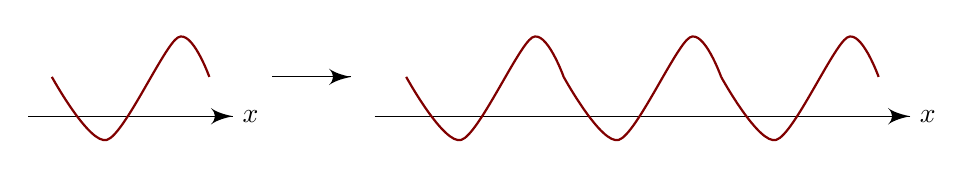
\begin{tikzpicture}
    \draw [->] (-0.3, 0) -- (2.3, 0) node [right] {$x$};
    \draw [mred, thick] plot [smooth] coordinates {(0, 0.5) (0.7, -0.3) (1.6, 1) (2, 0.5)};

    \draw [->] (2.8, 0.5) -- (3.8, 0.5);
    \draw [->] (4.1, 0) -- (10.9, 0) node [right] {$x$};
    \foreach \x in {4.5, 6.5, 8.5} {
      \draw [mred, thick] plot [smooth] coordinates {(\x, 0.5) (\x + 0.7, -0.3) (\x + 1.6, 1) (\x + 2, 0.5)};
    }
  \end{tikzpicture}
\end{center}
\subsection{Convergence of Fourier series}
When Fourier first proposed the idea of a Fourier series, people didn't really believe in him. How can we be sure that the infinite series actually converges? It turns out that in many cases, they don't.

To investigate the convergence of the series, we define the \emph{partial Fourier sum} as
\[
  S_n f = \sum_{m = -n}^n \hat{f}_m e^{im\theta}.
\]
The question we want to answer is whether $S_n f$ ``converges'' to $f$. Here we have to be careful with what we mean by convergence. As we (might) have seen in Analysis, there are many ways of defining convergence of functions. If we have a ``norm'' on the space of functions, we can define convergence to mean $\lim\limits_{n\to \infty}\|S_n f - f\| = 0$. Our ``norm'' can be defined as
\[
  \|S_n f - f\| = \frac{1}{2\pi}\int_{-\pi}^\pi \|S_n f(\theta) - f(\theta)\|^2 \;\d \theta.
\]
However, this doesn't really work if $S_n f$ and $f$ can be arbitrary functions, as in this does not necessarily have to be a norm. Indeed, if $\lim\limits_{n \to \infty}S_n f$ differs from $f$ on finitely or countably many points, the integral will still be zero. In particular, $\lim S_n f$ and $f$ can differ at all rational points, but this definition will say that $S_n f$ converges to $f$.

Hence another possible definition of convergence is to require
\[
  \lim_{n \to \infty}S_n f(\theta) - f(\theta) = 0
\]
for all $\theta$. This is known as \emph{pointwise convergence}. However, this is often too weak a notion. We can ask for more, and require that the \emph{rate} of convergent is independent of $\theta$. This is known as uniform convergence, and is defined by
\[
  \lim_{n \to \infty}\sup_{\theta} |S_n f(\theta) - f(\theta)| = 0.
\]
Of course, with different definitions of convergence, we can get different answers to whether it converges. Unfortunately, even if we manage to get our definition of convergence right, it is still difficult to come up with a criterion to decide if a function has a convergent Fourier Series. As of today, we still don't really understand how the convergence of Fourier series behaves.

Instead of trying to come up with something general, (since this is an applied course), let's look at an example instead.

\begin{eg}
  Consider the sawtooth function $f(\theta) = \theta$.
  \begin{center}
    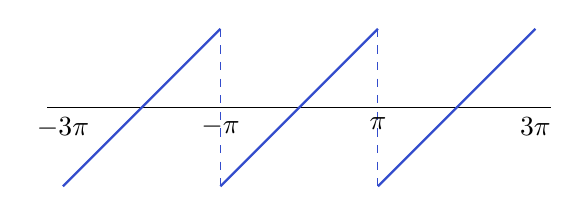
\begin{tikzpicture}
      \draw (-3.2, 0) -- (3.2, 0);

      \draw [thick, mblue] (-3, -1) -- (-1, 1);
      \draw [dashed, mblue] (-1, 1) -- (-1, -1);
      \draw [thick, mblue] (-1, -1) -- (1, 1);
      \draw [dashed, mblue] (1, 1) -- (1, -1);
      \draw [thick, mblue] (1, -1) -- (3, 1);

      \node at (-3, 0) [below] {$-3\pi$};
      \node at (-1, 0) [below] {$-\pi$};
      \node at (1, 0) [below] {$\pi$};
      \node at (3, 0) [below] {$3\pi$};
    \end{tikzpicture}
  \end{center}
  Note that this function is discontinuous at odd multiples of $\pi$.

  The Fourier coefficients (for $n \not= 0$) are
  \[
    \hat{f}_n = \frac{1}{2\pi}\int_{-\pi}^\pi e^{-in\theta}\theta\;\d \theta = \left[-\frac{1}{2\pi i n}e^{-in\theta}\theta\right]_{-\pi}^\pi + \frac{1}{2\pi i n}\int_{-\pi}^\pi e^{in\theta}\;\d \theta = \frac{(-1)^{n + 1}}{in}.
  \]
  We also have $\hat{f}_0 = 0$.

  Hence we have
  \[
    \theta = \sum_{n \not= 0}\frac{(-1)^{n + 1}}{in}e^{in\theta}.
  \]
  It turns out that this series converges to the sawtooth for all $\theta \not= (2m + 1)\pi$, ie. everywhere that the sawtooth is continuous.

  Let's look explicitly at the case where $\theta = \pi$. Each term of the partial Fourier series is zero. So we can say that the Fourier series converges to 0. This is the \emph{average} value of $\lim\limits_{\varepsilon \to 0} f(\pi \pm \varepsilon)$.

  This is typical. At an isolated discontinuity, the Fourier series is the average of the limiting values of the original function. as we approach from either side.
\end{eg}
\subsection{Differentiability and Fourier series}
Integration is a smoothening operator. If we take, say, the step function
\[
  \Theta(x) =
  \begin{cases}
    1 & x > 0\\
    0 & x < 0
  \end{cases}.
\]
Then the integral is given by
\[
  \int \Theta(x)\;\d x =
  \begin{cases}
    x & x > 0\\
    0 & x < 0
  \end{cases}.
\]
This is now a continuous function. If we integrate it again, we make the positive side look like a quadratic curve, and it is now differentiable.
\begin{center}
  \begin{tikzpicture}
    \draw [->] (-2, 0) -- (2, 0) node [right] {$x$};
    \draw [->] (0, -0.5) -- (0, 2.5) node [above] {$y$};
    \draw [mblue, thick] (-2, 0) -- (0, 0);
    \draw [mblue, thick] (0, 2) -- (2, 2);

    \draw [->] (2.5, 1) -- (3.5, 1) node [above, pos=0.5] {$\int\d x$};

    \draw [->] (4, 0) -- (8, 0) node [right] {$x$};
    \draw [->] (6, -0.5) -- (6, 2.5) node [above] {$y$};
    \draw [mred, thick] (4, 0) -- (6, 0);
    \draw [mred, thick] (6, 0) -- (8, 2);
  \end{tikzpicture}
\end{center}
On the other hand, when we differentiate a function, we generally make it worse. For example, when we differentiate the continuous function $\int \Theta (x)\;\d x$, we obtain the discontinuous function $\Theta(x)$. If we attempt to differentiate this again, we get the $\delta$-(non)-function.

Hence, it is often helpful to characterize the ``smoothness'' of a function by how many times we can differentiate it. It turns out this is rather relevant to the behaviour of the Fourier series.

Suppose that we have a function that is itself continuous and whose first $m - 1$ derivatives are also continuous, but $f^{(m)}$ has isolated discontinuities at $\{\theta_1, \theta_2, \theta_3, \cdots, \theta_r\}$.

We can look at the $k$th Fourier coefficient:
\begin{align*}
  \hat{f}_k &= \frac{1}{2\pi}\int_{-\pi}^\pi e^{-k\theta}f(\theta) \;\d \theta\\
  &= \left[-\frac{1}{2\pi i k}e^{-ik\theta}f(\theta)\right]^{\pi}_{-\pi} + \frac{1}{2\pi i k}\int_{-\pi}^\pi e^{-ik\theta}f'(\theta)\;\d \theta\\
  \intertext{The first term vanishes since $f(\theta)$ is continuous and takes the same value at $\pi$ and $-\pi$. So we are left with}
  &= \frac{1}{2\pi i k}\int_{-\pi}^\pi e^{-ik\theta}f'(\theta)\;\d \theta\\
  &= \cdots\\
  &= \frac{1}{(ik)^m}\frac{1}{2\pi} \int_{-\pi}^\pi e^{ik\theta} f^{(m)}(\theta)\;\d \theta.
  \intertext{Now we have to be careful, since $f^{(m)}$ is no longer continuous. However provided that $f^{(m)}$ is everywhere finite, we can approximate this by removing small strips $(\theta_i - \varepsilon, \theta_i + \varepsilon)$ from our domain of integration, and take the limit $\varepsilon \to 0$. We can write this as}
  &= \lim_{\varepsilon \to 0}\frac{1}{(ik)^m}\frac{1}{2\pi}\int_{-\pi}^{\theta_1 - \varepsilon} + \int_{\theta_1 + \varepsilon}^{\theta_2 - \varepsilon} + \cdots + \int_{\theta_r + \varepsilon}^{\pi} e^{ik\theta} f^{(m)}(\theta)\;\d \theta\\
  &= \frac{1}{(ik)^{m + 1}} \frac{1}{2\pi}\left[\sum_{s = 1}^r (f^{(m)}(\theta_s^+) - f^{(m)}(\theta_s^-)) + \int_{(-\pi, \pi)\setminus \theta} e^{-ik\theta} f^{(m + 1)}(\theta) \;\d \theta\right].
\end{align*}
We now have to stop. So $\hat{f}_k$ decays like $\left(\frac{1}{k}\right)^{m + 1}$ if our function and its $(m - 1)$ derivatives are continuous. This means that if a function is more differentiable, then the coefficients decay more quickly.

This makes sense. If we have a rather smooth function, then we would expect the first few Fourier terms (with low frequency) to account for most of the variation of $f$. Hence the coefficients decay really quickly.

However, if the function is jiggly and bumps around all the time, we would expect to need some higher frequency to account for the minute variation. Hence the terms would not decay away that quickly. Hence if we can differentiate it more times, then in general the terms should decay quicker.

\begin{thm}[Parseval's theorem]
  \[
    (f, f) = \int_{-\pi}^\pi |f(\theta)|^2 \;\d \theta = 2\pi \sum_{n\in \Z}|\hat{f}_n|^2
  \]
\end{thm}

\begin{proof}
  \begin{align*}
    (f, f) &= \int_{-\pi}^\pi |f(\theta)|^2 \;\d \theta\\
    &= \int_{-\pi}^{\pi} \left(\sum_{m \in \Z} \hat{f}_m^* e^{-im\theta}\right)\left(\sum_{n \in \Z} \hat{f}_n^* e^{-in\theta}\right)\;\d \theta\\
    &= \sum_{m, n\in \Z}\hat{f}_m^* \hat{f}_n \int_{-\pi}^\pi e^{i(m - n)\theta}\;\d \theta\\
    &= 2\pi \sum_{m, n\in \Z}\hat{f}_m^* \hat{f}_n \delta_{mn}\\
    &= 2\pi \sum_{n\in \Z}|\hat{f}_n|^n
  \end{align*}
\end{proof}
Note that this is not a fully rigorous proof, since we assumed not only that the Fourier series converges to the function, but also that we could commute the infinite sums. However, for the purposes of an applied course, this is sufficient.

Last time, we computed that the sawtooth function $f(\theta) = \theta$ has Fourier coefficients
\[
  \hat{f}_0 = 0,\quad \hat{f}_n = \frac{i(-1)^{n}}{n}\text{ for }n\not= 0.
\]
But why do we care? It turns out this has some applications in number theory. You might have heard of the Riemann $\zeta$-function, defined by
\[
  \zeta(s) = \sum_{n = 1}^\infty \frac{1}{n^s}.
\]
We will show that this obeys the property that for any $m$, $\zeta(2m) = \pi^{2m}q$ for some $q\in \Q$. This may not be obvious at first sight. So let's apply Parseval's theorem for the sawtooth. By direct computation, we know that
\[
  (f, f) = \int_{-\pi}^\pi \theta^2 \;\d \theta = \frac{2\pi^3}{3}.
\]
However, by Parseval's theorem, we know that
\[
  (f, f) = 2\pi \sum_{n \in \Z}|\hat{f}_n|^2 = 4\pi \sum_{n = 1}^\infty \frac{1}{n^2}.
\]
Putting these together, we learn that
\[
  \sum_{n = 1}^\infty \frac{1}{n^2} = \zeta(2) = \frac{\pi^2}{6}.
\]
We have just done it for the case where $m = 1$. But if we integrate the sawtooth function repeatedly, then we can get the general result for all $m$.

At this point, we might ask, why are we choosing these $e^{im\theta}$ as our basis? Surely there are a lot of different sets of basis we can use. For example, infinite dimensions, we can just arbitrary choose random vectors (that are not linearly dependent) to get a set of basis vectors. However, in practice, we don't pick them randomly. We often choose a basis that can reveal the symmetry of a system. For example, if we have a rotationally symmetric system, we would like to use polar coordinates. Similarly, if we have periodic functions, then $e^{im\theta}$ is often a good choice of basis.

\section{Sturm-Liouville Theory}
In finite dimensions, we often consider \emph{linear maps} $M: V\to W$. If $\{\mathbf{v}_i\}$ is a basis for $V$ and $\{\mathbf{w}\}$is a basis for $W$, then we can represent the map by a matrix with entries
\[
  M_{ai} = (\mathbf{w}_a, M\mathbf{v}_i).
\]
A map $M: V\to V$ is called \emph{self-adjoint} if $M^\dagger = M$ as matrices. However, it is not obvious how we can extend this notion to arbitrary maps between arbitrary vector spaces (with an inner product) when they cannot be represented by a matrix.

Instead, we can define the \emph{adjoint} $B$ of a map $A: V\to V$ to be a map such that
\[
  (B\mathbf{u}, \mathbf{v}) = (\mathbf{u}, A\mathbf{v})
\]
for all vectors $\mathbf{u}, \mathbf{v}\in V$. A map is then self-adjoint if
\[
  (M\mathbf{u}, \mathbf{v}) = (\mathbf{u}, M\mathbf{v}).
\]
Self-adjoint matrices come with a natural basis. Recall that the \emph{eigenvalues} of a matrix are the roots of $\det(M - \lambda I) = 0$. The \emph{eigenvector} corresponding to an eigenvalue $\lambda$ is defined by $M\mathbf{v}_i = \lambda_i \mathbf{v}_i$.

In general, eigenvalues can be any complex number. However, self-adjoint maps have \emph{real} eigenvalues. Suppose
\[
  M\mathbf{v}_i = \lambda_i \mathbf{v}_i.
\]
Then we have
\[
  \lambda_i (\mathbf{v}_i, \mathbf{v}_i) = (\mathbf{v}_i, M\mathbf{v}_i) = (M\mathbf{v}_i, \mathbf{v}_i) = \lambda_i^* (\mathbf{v}_i, \mathbf{v}_i).
\]
So $\lambda_i = \lambda_i^*$.

Furthermore, eigenvectors with distinct eigenvalues are orthogonal with respect to the inner product. Suppose that
\[
  M \mathbf{v}_i = \lambda_i \mathbf{v}_i,\quad M \mathbf{v}_j = \lambda_j \mathbf{v}_j.
\]
Then
\[
  \lambda_i (\mathbf{v}_j, \mathbf{v}_i) = (\mathbf{v}_j, M\mathbf{v}_i) = (M\mathbf{v}_j, \mathbf{v}_i) = \lambda_j(\mathbf{v}_j, \mathbf{v}_i).
\]
Since $\lambda_i \not= \lambda_j$, we must have $(\mathbf{v}_j, \mathbf{v}_i) = 0$.

Knowing eigenvalues and eigenvalues gives a neat way so solve linear equations of the form
\[
  M \mathbf{u} = \mathbf{f}.
\]
Here we are given $M$ and $\mathbf{f}$, and want to find $\mathbf{u}$. Of course, the answer is $\mathbf{u} = M^{-1}f$. However, if we expand in terms of eigenvectors, we obtain
\[
  M\mathbf{u} = M\sum u_i \mathbf{v}_i = \sum u_i \lambda_i \mathbf{v}_i.
\]
Hence we have
\[
  \sum u_i \lambda_i \mathbf{v}_i = \sum f_i \mathbf{v}_i.
\]
Taking the inner product with $\mathbf{v}_j$, we know that
\[
  u_j = \frac{f_j}{\lambda_j}.
\]
So far, these are all things from IA Vectors and Matrices. Sturm-Liouville theory is the infinite-dimensional analogue.

In our vector space of differentiable functions, our ``matrices'' would be linear differential operators $\mathcal{L}$. For example, we could have
\[
  \mathcal{L} = A_p(x) \frac{\d^p}{\d x^p} + A_{p - 1}(x) \frac{\d^{p - 1}}{\d x^{p - 1}} + \cdots + A_1(x)\frac{\d}{\d x} + A_0(x).
\]
It is an easy check that this is in fact linear.

We say $\mathcal{L}$ has order $p$ if the highest derivative that appears is $\frac{\d^p}{\d x^p}$.

In most applications, we will be interested in the case $p = 2$. When will our $\mathcal{L}$ be self-adjoint?

In the $p = 2$ case, we have
\begin{align*}
  \mathcal{L} y &= P \frac{\d^2 y}{\d x^2} + R \frac{\d y}{\d x} - Q y \\
  &= P\left[\frac{\d^2 y}{\d x^2} + \frac{R}{P}\frac{\d y}{\d x} - \frac{Q}{P}y\right] \\
  &= P\left[e^{-\int \frac{R}{P}\;\d x}\frac{\d}{\d x}\left(e^{\int \frac{R}{P}\;\d x}\frac{\d y}{\d x}\right)- \frac{Q}{P}y\right]\\
  \intertext{Let $p = \exp\left(\int \frac{R}{P}\;\d x\right)$. Then we can write this as}
  &= P p^{-1}\left[\frac{\d}{\d x}\left(p\frac{\d y}{\d x}\right) - \frac{Q}{P}p y\right].
\end{align*}
We further define $q = \frac{Q}{P}p$. We also drop a factor of $Pp^{-1}$. Then we are left with
\[
  \mathcal{L} = \frac{\d}{\d x}\left(p(x)\frac{\d}{\d x}\right) - q(x).
\]
This is the \emph{Sturm-Liouville form} of the operator. Now let's compute $(f, \mathcal{L}g)$. We integrate by parts numerous times to obtain
\begin{align*}
  (f, \mathcal{L}g) &= \int_a^b f^*\left(\frac{\d}{\d x}\left(p \frac{\d g}{\d x}\right) - qg\right)\;\d x \\
  &= [f^* pg']_a^b - \int_a^b \left(\frac{\d f^*}{\d x}p\frac{\d g}{\d x} + f^* qg\right)\;\d x\\
  &= [f^*pg' - f'^*pg]_a^b + \int_a^b \left(\frac{\d}{\d x}\left(p\frac{\d f^*}{\d x}\right) - qf^*\right)g\;\d x\\
  &= [(f^*g' - f'^*g)p]_a^b + (\mathcal{L}f, g),
\end{align*}
assuming that $p, q$ are real.

So 2nd order linear differential operators are self-adjoint with respect to this norm if $p, q$ are real and the boundary terms vanish. When do the boundary terms vanish? One possibility is when $p$ is periodic (with the right period), or if we constrain $f$ and $g$ to be periodic.

\begin{eg}
  We can consider a simple case, where
  \[
    \mathcal{L} = \frac{\d^2}{\d x^2}.
  \]
  Here we have $p = 1, q = 0$. If we ask for functions to be periodic on $[a, b]$, then
  \[
    \int_a^b f^*\frac{\d^2 g}{\d x^2}\;\d x = \int_a^b \frac{\d^2 f^*}{\d x^2}g\;\d x.
  \]
  Note that it is important that we have a \emph{second-order} differential operator. If it is first-order, then we would have a negative sign, since we integrated by parts once.
\end{eg}

Just as in finite dimensions, self-adjoint operators have eigenfunctions and eigenvalues with special properties. First, we define a more sophisticated inner product.
\begin{defi}[Inner product with weight]
  An \emph{inner product with weight} $w$, written $(\cdot, \cdot)_w$, is defined by
  \[
    (f, g)_w = \int_a^b f^*(x) g(x) w(x)\;\d x,
  \]
  where $w$ is real, non-negative, and has only finitely many zeroes.
\end{defi}
Why do we want a weight $w(x)$? In the future, we might want to work with the unit disk, instead of a square in $\R^2$. When we want to use polar coordinates, we will have to integrate with $r\;\d r\;\d \theta$, instead of just $\d r\;\d \theta$. Hence we need the weight of $r$. Also, we allow it to have finitely many zeroes, so that the radius can be $0$ at the origin.

Why can't we have more zeroes? We want the inner product to keep the property that $(f, f)_w = 0$ iff $f = 0$ (for continuous $f$). If $w$ is zero at too many places, then the inner product could be zero without $f$ being zero.

We now define what it means to be an eigenfuction.
\begin{defi}[Eigenfunction with weight]
  An \emph{eigenfunction with weight} $w$ of $\mathcal{L}$ is a function $y: [a, b] \to \C$ obeying the differential equation
  \[
    \mathcal{L} y = \lambda w y,
  \]
  where $\lambda\in \C$ is the eigenvalue.
\end{defi}
This might be strange at first sight. It seems like we can take any nonsense $y$, apply $\mathcal{L}$, to get some nonsense $\mathcal{L} y$. But then it is fine, since we can write it as some nonsense $w$ times our original $y$. So any function is an eigenfunction? No! There are many constraints $w$ has to satisfy, like being positive, real and having finitely many zeroes. It turns out this severely restraints what values $y$ can take, so not everything will be an eigenfunction. In fact we can develop this theory without the weight function $w$. However, weight functions are much more convenient when, say, dealing with the unit disk.

\begin{prop}
  The eigenvalues of a Sturm-Liouville operator are real.
\end{prop}

\begin{proof}
  Suppose $\mathcal{L} y_i = \lambda_i w y_i$. Then
  \[
    \lambda_i (y_i, y_i)_w = \lambda_i (y_i, w y_i) = (y_i, \mathcal{L} y_i) = (\mathcal{L} y_i, y_i) = (\lambda_i w y_i, y_i) = \lambda_i^* (y_i, y_i)_w.
  \]
  Since $(y_i, y_i)_w \not= 0$, we have $\lambda_i = \lambda_i^*$.
\end{proof}
Note that the first and last terms use the weighted inner product, but the middle terms use the unweighted inner product.

\begin{prop}
  Eigenfunctions with different eigenvalues (but same weight) are orthogonal.
\end{prop}

\begin{proof}
  Let $\mathcal{L} y_i = \lambda_i w y_i$ and $\mathcal{L} y_j = \lambda_j w y_j$. Then
  \[
    \lambda_i (y_j, y_i)_w = (y_j, \mathcal{L} y_i) = (\mathcal{L} y_j, y_i) = \lambda_j (y_j, y_i)_w.
  \]
  Since $\lambda_i \not= \lambda_j$, we must have $(y_j, y_i)_w = 0$.
\end{proof}

\begin{prop}
  On a \emph{compact} domain, the eigenvalues $\lambda_1, \lambda_2, \cdots$ form a countably infinite sequence and are discrete.
\end{prop}
We will not prove this.

This will be a rather helpful result in quantum mechanics, since in quantum mechanics, the possible values of, say, the energy are the eigenvalues of the Hamiltonian operator. Then this result says that the possible values of the energy are discrete and form an infinite sequence.

Note here the word \emph{compact}. In quantum mechanics, if we restrict a particle in a well $[0, 1]$, then it will have quantized energy level since the domain is compact. However, if the particle is free, then it can have any energy at all since we no longer have a compact domain. Similarly, angular momentum is quantized, since it describe rotations, which takes values in $S^1$, which is compact.

\begin{prop}
  The eigenfunctions are complete: any function $f: [a, b] \to \C$ (obeying appropriate boundary conditions) can be expanded as
  \[
    f(x) = \sum_n f_n y_n(x),
  \]
  where
  \[
    \hat{f}_n = \int y^*_n(x) f(x) w(x)\;\d x.
  \]
\end{prop}

\begin{eg}
  Let $[a, b] = [-L, L]$, $\mathcal{L} = \frac{\d^2}{\d x^2}$, $w = 1$, restricting to periodic functions Then our eigenfunction obeys
  \[
    \frac{\d^2 y_n}{\d x^2} = \lambda_n y_n(x),
  \]
  Then our periodic functions are
  \[
    y_n(x) = \exp\left(\frac{in\pi x}{L}\right)
  \]
  with eigenvalues 
  \[
    \lambda_n = - \frac{n^2 \pi^2}{L^2}
  \]
  for $n \in \Z$. This is just the Fourier series!
\end{eg}

\begin{eg}[Hermite polynomials]
  We are going to cheat a little bit and pick our domain to be $\R$. We want to study the differential equation
  \[
    \frac{1}{2}H'' - xH' = \lambda H,
  \]
  with $H: \R \to \C$. We want to put this in Sturm-Liouville form. We have
  \[
    p(x) = \exp\left(-\int_0^x 2t \;\d t\right) = e^{-x^2},
  \]
  ignoring constant factors. Then $q(x) = 0$. We can rewrite this as
  \[
    \frac{\d}{\d x}\left(e^{-x^2}\frac{\d H}{\d x}\right) = -2\lambda e^{-x^2} H(x).
  \]
  So we take our weight function to be $w(x) = e^{-x^2}$.

  We now ask that $H(x)$ grows at most polynomially as $|x| \to \infty$. In particular, we want $e^{-x^2}H(x)^2 \to 0$. This ensures that the boundary terms from integration by parts vanish at the infinite boundary, so that our Sturm-Liouville operator is self-adjoint.

  The eigenfunctions turn out to be
  \[
    H_n(x) = (-1)^n e^{x^2}\frac{\d^n}{\d x^n}\left(e^{-x^2}\right).
  \]
  These are known as the \emph{Hermite polynomials}. Note that these are indeed polynomials. When we differentiate the $e^{-x^2}$ term many times, we get a lot of things from the product rule, but they will always keep an $e^{-x^2}$, which will ultimately cancel with $e^{x^2}$.
\end{eg}

Just as for matrices, we can use the eigenfunction expansion to solve forced differential equations. For example, if might want to solve
\[
  \mathcal{L} g = f(x),
\]
where $f(x)$ is a forcing term. We can write this as
\[
  \mathcal{L} g = w(x) F(x).
\]
We exapnd our $g$ as
\[
  g(x) = \sum_{n \in \Z}\hat{g}_n y_n(x).
\]
Then by linearity, 
\[
  \mathcal{L}g = \sum_{n \in \Z}\hat{g}_n \mathcal{L} y_n(x) = \sum_{n \in \Z}\hat{g}_n \lambda_n w(x)y_n(x).
\]
We can also expand our forcing functionas
\[
  w(x) F(x) = w(x) \left(\sum_{n \in \Z}\hat{F}_n y_n(x)\right).
\]
Taking the (regular) inner product with $y_m(x)$ (and noting orthogonality of eigenfunctions), we obtain
\[
  w(x) \hat{g}_m \lambda_m = w(x) \hat{F}m
\]
This tells us that
\[
  \hat{g}_m = \frac{\hat{F}_m}{\lambda_m}.
\]
So we have
\[
  g(x) = \sum_{n \in \Z}\frac{\hat{F}_n}{\lambda_n}y_n(x),
\]
provided all $\lambda_n$ are non-zero.

This is a systematic way of solving forced differential equations. We used to solve these by ``being smart''. We just looked at the forcing term and tried to guess what would work. Unsurprisingly, this approach does not suceed all the time. Thus it is helpful to have a systematic way of solving the equations.

It is often helpful to rewrite this into another form, using the fact that $\hat{F}_n = (y_n, F)_w$. So we have
\[
  g(x) = \sum_{n \in \Z}\frac{1}{\lambda_n}(y_n, F)_w y_n(x) = \int_a^b \sum_{n \in \Z}\frac{1}{\lambda_n} y_n^*(t) y_n(x) w(t) F(t)\;\d t.
\]
Note that we swapped the sum and the integral, which is in general a dangerous thing to do, but we don't really care because this is an applied course. We can further write the above as
\[
  g(x) = \int_a^b G(x, t) F(t) w(t)\;\d t,
\]
where $G(x, t)$ is the infinite sum
\[
  G(x, t) = \sum_{n \in \Z}\frac{1}{\lambda_n}y_n^*(t) y_n(x).
\]
Note that this depends on $\lambda_n$ and $y_n$ only. It depends on the differential operator $\mathcal{L}$, but not the forcing term $F$. We can think of this as something like the ``inverse matrix'', which we can use to solve the forced differential equation for any forcing term.
\end{document}
